% !TeX spellcheck = en_US
\documentclass[12pt,fleqn]{article}


\usepackage[english]{babel}

\usepackage{texfiles/SpeedyGonzales}
\usepackage{texfiles/MediocreMike}
\usepackage{verbatim} 













\title{Bayesian Optimization for Hyperparameter Tuning in The Fully Connected Layers of VGG16}
\author{Søren Winkel Holm\and Oskar Wiese\and Anders Henriksen\and Anne Agathe Pedersen}
\date{\today}

\fancypagestyle{plain}
{
	\fancyhf{}
	\rfoot{Page \thepage{} of  \pageref{LastPage}}
	\renewcommand{\headrulewidth}{0pt}
}
%\pagestyle{fancy}
%\fancyhf{}
%\lhead{Lala}
%\chead{}
%\rhead{}
%\rfoot{Page \thepage{} of \pageref{LastPage}}

\graphicspath{{imgs/}}
\usepackage{float}
\usepackage[caption = false]{subfig}
%\linespread{1.15}

%TODO: \numberwithin{equation}{section}
%TODO: \numberwithin{footnote}{section}
%TODO: \numberwithin{figure}{section}
%TODO: \numberwithin{table}{section}

\begin{document}






\maketitle

%\tableofcontents
%\thispagestyle{fancy}
%\tableofcontents

\begin{abstract}
\noindent Optimization of neural network hyper parameters is a costly process of uncertainty balancing exploration of parameters and exploitation of known results. This experiment compares Bayesian Optimization using Gaussian Processes to  simple grid search for finding the optimal hyper parameters for the fully-connected layers of the VGG16 image classification deep convolutional network. The training is compared using three different acquisitions functions and. Little difference is found which could be a result of the limited scope of the network training but the Bayesian Optimization method allows for a visualization of the estimated model accuracy on the hyper parameter space.

\end{abstract}


\section{Introduction} 
Development of effective machine learning models has spawned a vision of generalizable machine intelligence which can replace the comparatively slower and more erronoeus human work in many fields. While this generalizability is often true, the popular deep models have one glaring issue that requires skill and tonnes of computing power to overcome; hyperparameter optimization. Optimizing the hyperparameters usually devolves into random guessing, though new methods are on the rise like Bayesian optimization, which greatly reduces the effort involved in finding the parameters with use of an acquisition function and probabilistic model.

In this paper, Bayesian optimization with Gaussian processes as probabilistic model and expected improvement, upper confidence bound and probability of improvement as acquisition function will be used to find the hyperparameters of the VGG16 classifier network when training to classify on the 10 classes of the CIFAR10 dataset, optimizing for the validation accuracy.


\section{Methods}
Bayesian optimization of hyperparameters is carried out by building a probabilistic model of the objective function and then using these probabilities to select the most likely values of hyperparameters to evaluate the true objective function on. After more and more evaluations, the surrogate model will become an increasingly better approximation of the true function. 

\subsection*{Gaussian Process}
In Bayesian optimization, Gaussian Processes (GPs) are used as a non-parametric approach to finding the distribution over functions that are still consistent with the observed data. Hence, the mean of this distribution will be the most probable fit of the data. It should be noted that GPs assume smoothness of the data, meaning that if $x_1$ produces $y_1$, a point $x_2$ close to $x_1$ should produce a $y_2$ close to $y_1$. 

\subsection*{Acquisition Functions}

\subsubsection*{Probability of Improvement (PI)}
PI evaluates the objective function, \textit{f}, at the point most likely to improve the minimum value. In this project, PI evaluates at the point most likely to obtain a higher accuracy, since the function is given the negative accuracy. PI is evaluated by
\begin{equation*}
	\text{PI}(\mathbf{x}) = \text{P}(f(\mathbf{x}) \geq f(\mathbf{x}^+) + \xi) 
	= \Phi\biggl(\frac{\mu(\mathbf{x}) - f(\mathbf{x}^+) - \xi}{\sigma(\mathbf{x})}\biggr),
\end{equation*}
\noindent
where $\xi$ is an explore/exploit trade-off variable and $\Phi$ is the gaussian CDF.

\subsubsection*{Expected Improvement (EI)}
EI tries to quantify the improvement instead of the probability of improving as PI does. It is possible to quantify the average value of improvement if we sample the objective function at $x$. The acquisition function then computes the expected value of the improvement function at a certain x. EI is expressed as 
\begin{equation*}
\mathrm{EI}(\mathbf{x})=\left\{\begin{array}{ll}
\left(\mu(\mathbf{x})-f\left(\mathbf{x}^{+}\right)\right) \Phi(Z)+\sigma(\mathbf{x}) \phi(Z) & \text { if } \sigma(\mathbf{x})>0 \\
0 & \text { if } \sigma(\mathbf{x})<0,
\end{array}\right. 
\end{equation*}
where $ Z = \frac{\mu(\mathbf{x}) - f(\mathbf{x}^+) - \xi }{\sigma(\mathbf{x})}$ \newline 

\subsubsection*{Gaussian Process Upper Confidence Bound(GP-UCB)}
The idea behind GP-UCB is to directly use the mean and variance from the Gaussian distribution. These two parameters are used as the exploration / exploitation trade off. The function is given as
\begin{equation*}
UCB(x) = \mu(x) + \kappa \sigma(x),
\end{equation*}
\noindent
Where $ \kappa $ controls the explore/exploit trade-off. \newline

\subsection*{Grid Search}

Grid search is a commonplace way of performing hyperparameter tuning by exhaustively searching the parameter space. In this project, grid search explores these parameters:\\
	\indent \indent \texttt{hidden = np.array([100,2000,4000]) ; drop = np.array([0.33, 0.66])\\
 \indent \indent activ\_func = {Tanh, ReLU, ReLU6, Sigmoid} } \\
This implementation constructs 12 models, which is the same amount as the number of GP iterations. 

\section{Results}

\begin{table}[H]\label{resultater}
	\begin{tabular}{l|lllll}
		  & Opt. hidden units & Opt. dropout \textit{p} & Opt. activation & Val. accuracy &Test accuracy \\ \hline
		BO: EI  & 2540      & 16\pro              & Tanh             &    62.8\pro & 61.7\pro   \\ 
		BO: MPI & 2403         & 61\pro             & Sigmoid             & 64.7\pro  & 63.1\pro     \\ 
		BO: UCB & 1150         & 53\pro              & Sigmoid             & 64.6\pro  & 64.4\pro     \\ 
		Grid search & 2000         & 66\pro              & Sigmoid             & 64.9\pro & 63.1\pro          \\
	\end{tabular}
	\caption{The optimal hyperparameters from running bayesian optimization with all three acquisition functions as well as grid search. All iterations can be seen in the appendix.}
\end{table}
\begin{figure}[H]
	\centering

	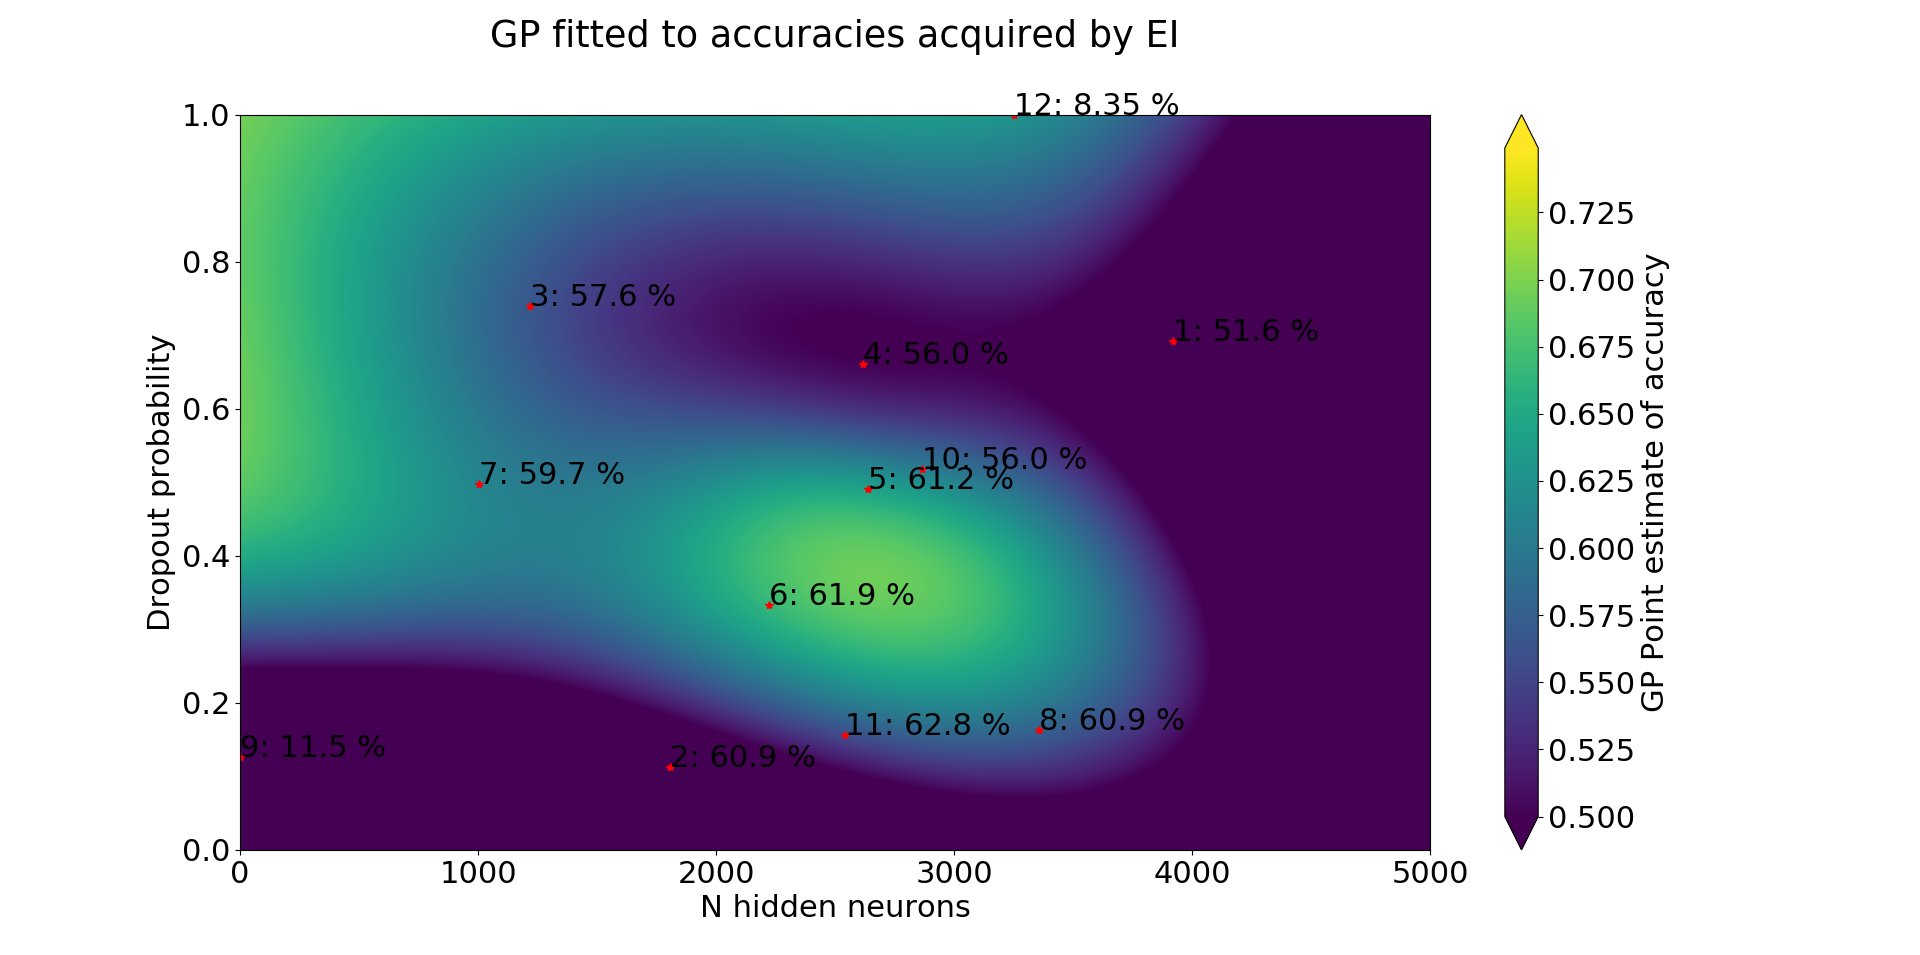
\includegraphics[width=\textwidth]{EIGP}	

\caption{The Gaussian process fitted to the twelve accuracy points acquired by the expected improvement function. The other GP visualizations can be seen in the appendix.}
%It is clear that especially the sixth iteration of the grid search happens to hit points where the GP finds accuracy peaks. 
\end{figure}
\section{Discussion}
%In this section you interpret your findings and describe why they are important and how they fit in with
%other research. You can also mention ways your study could have been improved and future areas of
%research.
% What might the answer imply, and what does it matter?
% How does it fit in with what other researchers have found?
% What are the perspectives for future research? 

From the table seen in results \ref{resultater}, Bayesian optimization has proposed hyperparameters that makes the accuracy higher than the hyperparameters found using grid search. However, the difference in accuracies between the model proposed by Bayesian optimization and grid search are $ \Delta p = 0.011$. To see if there is an actual significant difference between the accuracy of the models, a McNemar test can be performed. This is beyond the scope of this project and will be left for future work. In reality a McNemar test would probably show that there is no significant difference between the accuracy of the two models. Hence, this shows that a random search grid and Bayesian optimization finds hyperparameters for VGG16 that are equally good.
\\\\
When using the Bayesian optimization with GPyOpt, the first five iterations are purely exploration runs. Which means that in this project, Bayesian optimization only has seven iterations to choose the right direction in the parameter space to find the optimal parameters for VGG16. Due to the short amount of training time used in this project, an emerged challenge is to find parameters that makes VGG16 converge fast. However, this is not necessarily the optimal way of finding parameters that yields the highest possible accuracy of the network, as it is possible that there exists parameters that requires longer training for VGG16 to converge.
\\\\
The results discovered in this project shows that Bayesian optimization can be used for hyperparameter tuning. The advantage of Bayesian optimization compared to grid search, is that Bayesian optimization does not need to explore the whole parameter space because it believes certain areas do not contain parameters that maximizes the accuracy of VGG16. This limits the amount of time used for tuning the parameters of the the model compared to grid search which in turn searches the whole parameter space.

\section{References}
\url{https://gpyopt.readthedocs.io/en/latest/index.html}
\section{Appendix}
\begin{figure}[H]

		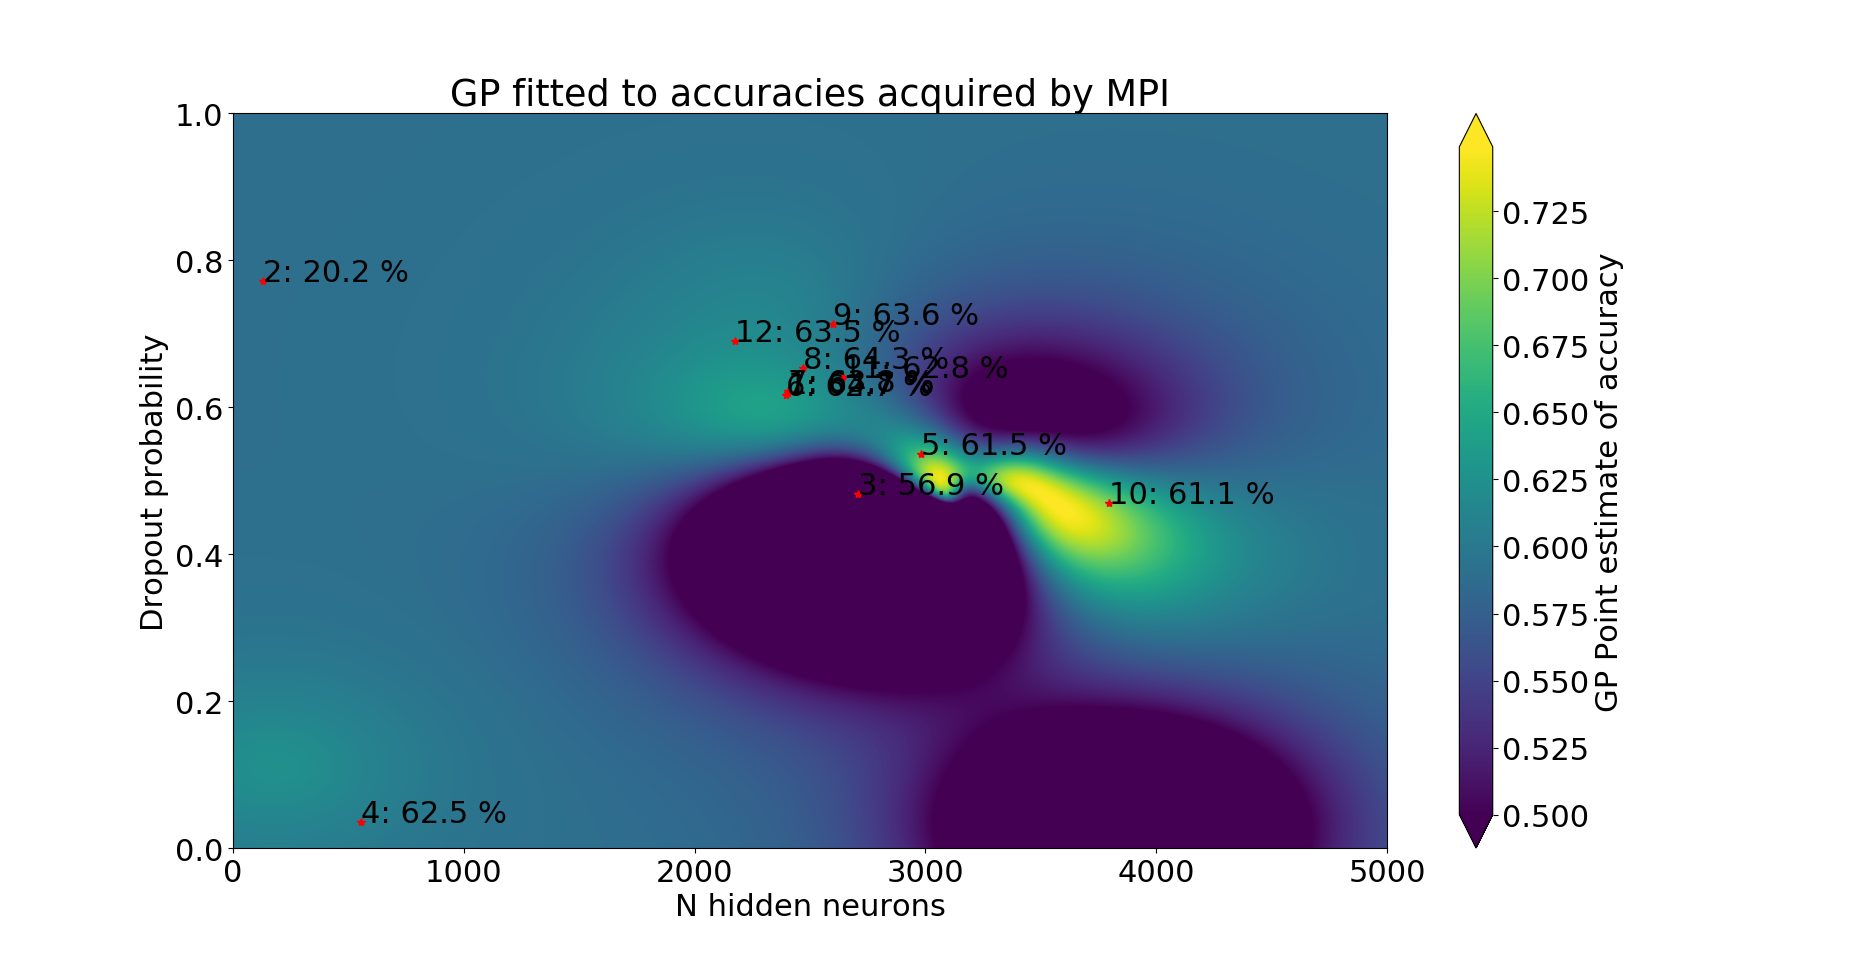
\includegraphics[width=\textwidth]{MPIGP}	
\end{figure}
\begin{figure}[H]
		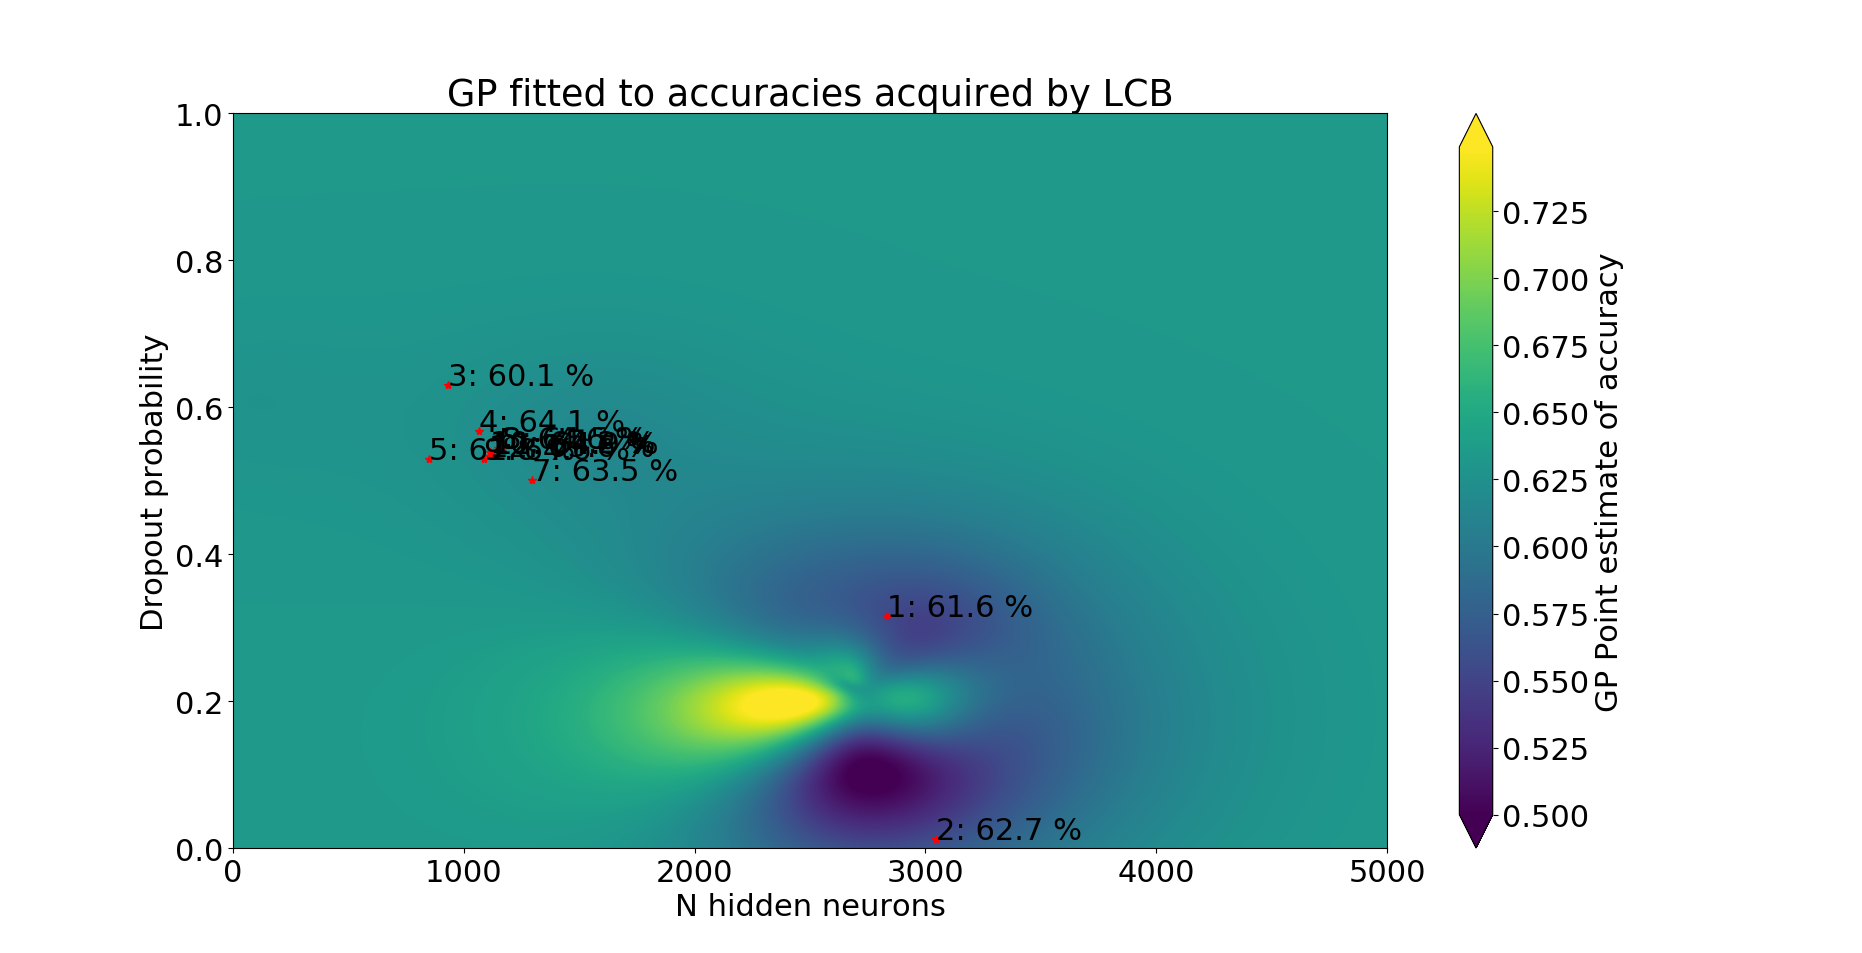
\includegraphics[width=\textwidth]{LCBGP}	

\end{figure}
\begin{table}[H]
	\caption{Bayesian optimization with EI as acquisition function \label{EI}}
	\centering
	\begin{tabular}{|l|l|l|l|l|}
		\hline
		Iteration & Hidden units & Dropout probability & Activation function & Accuracy \\ \hline
		1 & 3917 & 0.6923 & ReLU & 0.5165 \\ \hline 

		2 & 1805 & 0.1127 & Tanh & 0.6091 \\ \hline 

		3 & 1217 & 0.7398 & ReLU6 & 0.5765 \\ \hline 

		4 & 2618 & 0.6605 & ReLU & 0.5605 \\ \hline 

		5 & 2639 & 0.491 & Tanh & 0.6115 \\ \hline 

		6 & 2220 & 0.3325 & Tanh & 0.6185 \\ \hline 

		7 & 1002 & 0.4978 & Tanh & 0.5965 \\ \hline 

		8 & 3354 & 0.1637 & Tanh & 0.6091 \\ \hline 

		9 & 1 & 0.1262 & ReLU & 0.1145 \\ \hline 

		10 & 2863 & 0.5179 & Tanh & 0.5595 \\ \hline 

		11 & 2540 & 0.1569 & Tanh & 0.6275 \\ \hline 

		12 & 3251 & 1.0 & ReLU6 & 0.0835 \\ \hline 

	\end{tabular}
\end{table}
\begin{table}[H]
	\caption{Bayesian optimization with MPI as acquisition function \label{MPI}}
	\centering
	\begin{tabular}{|l|l|l|l|l|}
		\hline
		Iteration & Hidden units & Dropout probability & Activation function & Accuracy \\ \hline
1 & 2403 & 0.6196 & Sigmoid & 0.647 \\ \hline 

2 & 130 & 0.7724 & ReLU & 0.202 \\ \hline 

3 & 2706 & 0.4818 & Tanh & 0.5685 \\ \hline 

4 & 554 & 0.03571 & ReLU6 & 0.6245 \\ \hline 

5 & 2983 & 0.5369 & ReLU & 0.6145 \\ \hline 

6 & 2397 & 0.6166 & Sigmoid & 0.6275 \\ \hline 

7 & 2407 & 0.6219 & Sigmoid & 0.6385 \\ \hline 

8 & 2471 & 0.6537 & Sigmoid & 0.6435 \\ \hline 

9 & 2601 & 0.7138 & Sigmoid & 0.6367 \\ \hline 

10 & 3794 & 0.4693 & ReLU & 0.6113 \\ \hline 

11 & 2641 & 0.6416 & Sigmoid & 0.6285 \\ \hline 

12 & 2176 & 0.69 & Sigmoid & 0.6355 \\ \hline 

	\end{tabular}
\end{table}



\begin{table}[H]
	\caption{Bayesian optimization with LCB as acquisition function \label{LCB}}
	\centering
	\begin{tabular}{|l|l|l|l|l|}
		\hline
		Iteration & Hidden units & Dropout probability & Activation function & Accuracy \\ \hline
		1 & 2835 & 0.316 & ReLU6 & 0.6162 \\ \hline 
		2 & 3046 & 0.01182 & Sigmoid & 0.627 \\ \hline 
		3 & 934 & 0.6308 & Tanh & 0.6005 \\ \hline 
		4 & 1068 & 0.5681 & Sigmoid & 0.641 \\ \hline 
		5 & 848 & 0.5295 & ReLU & 0.6175 \\ \hline 
		6 & 1150 & 0.5441 & Sigmoid & 0.646 \\ \hline 
		7 & 1297 & 0.5009 & Sigmoid & 0.635 \\ \hline 
		8 & 1165 & 0.5443 & Sigmoid & 0.6455 \\ \hline 
		9 & 1089 & 0.5296 & Sigmoid & 0.646 \\ \hline 
		10 & 1115 & 0.5386 & Sigmoid & 0.6425 \\ \hline 
		11 & 1127 & 0.5375 & Sigmoid & 0.649 \\ \hline 
		12 & 1112 & 0.5333 & Sigmoid & 0.636 \\ \hline 
	\end{tabular}
\end{table}
 
 
\begin{table}[H]
	\caption{Grid search \label{grid}}
	\centering
	\begin{tabular}{|l|l|l|l|l|}
		\hline
		Iteration & Hidden units & Dropout probability & Activation function & Validation loss \\ \hline
		1         & 100          & 0.33                & Sigmoid             & 0.6345          \\ \hline
		2         & 100          & 0.33                & Sigmoid             & 0.6405          \\ \hline
		3         & 100          & 0.66                & ReLU                & 0.5150          \\ \hline
		4         & 100          & 0.66                & Sigmoid             & 0.5610          \\ \hline
		5         & 2000         & 0.33                & Tanh                & 0.513           \\ \hline
		6         & 2000         & 0.33                & ReLU                & 0.649           \\ \hline
		7         & 2000         & 0.66                & Sigmoid             & 0.6525          \\ \hline
		8         & 2000         & 0.66                & ReLU6               & 0.5685          \\ \hline
		9         & 4000         & 0.33                & Tanh                & 0.5595          \\ \hline
		10        & 4000         & 0.33                & ReLU6               & 0.5345          \\ \hline
		11        & 4000         & 0.66                & ReLU6               & 0.5015          \\ \hline
		12        & 4000         & 0.66                & Tanh                & 0.5050          \\ \hline
	\end{tabular}
\end{table}

\end{document}

















